\chapter{Cesium代码解析}

\section{基本原理}
\begin{enumerate}
	\item 初始状态:从太空中远眺地球,将看到的地球三维场景绘制在平面画布上。每秒保持60帧的频率不断渲染画布。
	      \begin{figure}[!htb]
		      \centering
		      
\includegraphics[width=0.6\textwidth]{./charpter2/base/global.png}
	      \end{figure}
	\item 交互状态:当用户人机交互(放大/缩小)改变了视角后,由于每一帧都会重绘画布,让用户感觉是自己主动更新了画布一般,实际上是通过高频率的被动渲染来实现的。
\end{enumerate}

\subsection{核心代码}

\begin{enumerate}
	\item 轮询主入口 Source/Core/\textbf{requestAnimationFrame.js}。这个是封装js自身的requestAnimationFrame.js的requestAnimationFrame的缺陷在于只能通过window上下文来invoke回调,需要实现一种脱离window上下文的封装。
	\item 场景组件 Source/Widgets/CesiumWidget/\textbf{CesiumWidget.js} 用来呈现三维球场景的DOM场景组件。
	      \begin{figure}[!htb]
		      \centering
		      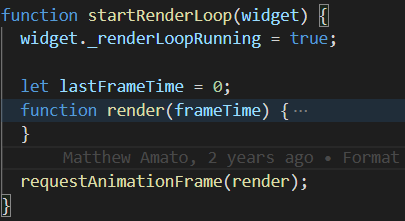
\includegraphics[width=0.5\textwidth]{./charpter2/base/loop.png}
	      \end{figure}
	      \begin{enumerate}
		      \item 构造函数内部逻辑
		            \begin{enumerate}
			            \item 初始化规定的椭球Ellipsoid,默认是WGS84
			            \item 初始化天空盒、月亮、太阳、大气环境
			            \item 初始化基本的栅格底图
			            \item 初始化基本的地形
			            \item 执行核心渲染进程,启动每秒60帧的轮询进程
		            \end{enumerate}

	      \end{enumerate}
	\item 核心渲染进程 Source/Scene/\textbf{Scene.js}
	      \begin{enumerate}
		      \item 先进入Scene的initializeFrame以及render函数
		      \item 先进入Scene的render函数是整个场景的主入口,内部会进行对应的各种不同图层的任务分发与调度,代码如下所示
		            \begin{lstlisting}
scene.globe.beginFrame(frameState); // 一帧的开始

scene.updateEnvironment();
// 只考虑球面模式实际是executeCommandsInViewport在工作
scene.updateAndExecuteCommands(passState, backgroundColor); 
scene.resolveFramebuffers(passState);

passState.framebuffer = undefined;
executeOverlayCommands(scene, passState);

scene.globe.endFrame(frameState); // 一帧的结束
\end{lstlisting}
	      \end{enumerate}
	\item 地形渲染 Source/Scene/\textbf{Globe.js}
	      \begin{enumerate}
		      \item 地形渲染的入口是Globe.js,其核心的工作类是surface,其构造函数如下:
		            \begin{lstlisting}
			// 默认采取四叉树构建表面	
			this._surface = new QuadtreePrimitive({ 
				tileProvider: new GlobeSurfaceTileProvider({
					terrainProvider: terrainProvider, // 一份地形
					imageryLayers: imageryLayerCollection, // 一组栅格瓦片底图
					surfaceShaderSet: this._surfaceShaderSet
				})
			});
		\end{lstlisting}
		      \item 地形的渲染是通过Globe.render beginFrame endFrame,三者共同组成其声明周期。
		            \begin{enumerate}
			            \item \textbf{beginFrame}函数原理
			                  \begin{lstlisting}
				QuadtreePrimitive.prototype.beginFrame = function (frameState) {
					var passes = frameState.passes;
					if (!passes.render) {
						return;
					}
				
					if (this._tilesInvalidated) {
						invalidateAllTiles(this);
						this._tilesInvalidated = false;
					}
				
					// Gets commands for any texture re-projections
					this._tileProvider.initialize(frameState);
				
					clearTileLoadQueue(this);
				
					if (this._debug.suspendLodUpdate) {
						return;
					}
				
					this._tileReplacementQueue.markStartOfRenderFrame();
				};
			\end{lstlisting}
			                  \begin{tikzpicture}
				                  \begin{umlseqdiag}
					                  \umlobject[class=Scene]{S}
					                  \umlobject[class=Globe]{G}
					                  \umlobject[class=QuadtreePrimitive]{surface}
					                  \umlobject[class=GlobeSurfaceTileProvider]{t}
					                  \begin{umlcall}{S}{G}
						                  \begin{umlcall}[op=beginFrame(),type=synchron,return=0]{G}{surface}
							                  \begin{umlcall}[type=synchron,fill=green]{surface}{t}
								                  \begin{umlcallself}[op=setTerrainProvidertype=synchron,fill=green]{t}
								                  \end{umlcallself}
							                  \end{umlcall}
							                  \begin{umlcallself}[op=start-beginFrame,type=synchron,fill=blue,return=end-beginFrame]{surface}
								                  \begin{umlcall}[op=initialize,type=synchron,fill=blue]{surface}{t}
								                  \end{umlcall}
								                  \begin{umlcallself}[op=clearTileLoadQueue,type=synchron,fill=blue]{surface}
								                  \end{umlcallself}
								                  \begin{umlcallself}[op=markStartOfRenderFrame,type=synchron,fill=blue]{surface}
								                  \end{umlcallself}
							                  \end{umlcallself}
						                  \end{umlcall}
					                  \end{umlcall}
				                  \end{umlseqdiag}
			                  \end{tikzpicture}
			            \item \textbf{render}函数原理
			                  \begin{lstlisting}
							QuadtreePrimitive.prototype.render = function (frameState) {
							var passes = frameState.passes;
							var tileProvider = this._tileProvider;

							if (passes.render) {
								tileProvider.beginUpdate(frameState);

								selectTilesForRendering(this, frameState);
								createRenderCommandsForSelectedTiles(this, frameState);

								tileProvider.endUpdate(frameState);
							}

							if (passes.pick && this._tilesToRender.length > 0) {
								tileProvider.updateForPick(frameState);
							}
						};
						\end{lstlisting}
			                  \begin{tikzpicture}
				                  \begin{umlseqdiag}
					                  \umlobject[class=Scene]{S}
					                  \umlobject[class=Globe]{G}
					                  \umlobject[class=QuadtreePrimitive]{surface}
					                  \umlobject[class=GlobeSurfaceTileProvider]{t}
					                  \begin{umlcall}{S}{G}
						                  \begin{umlcall}[op=render(),type=synchron,return=0]{G}{surface}
							                  % \begin{umlcall}[type=synchron,fill=green]{surface}{t}
							                  % 	\begin{umlcallself}[op=setTerrainProvidertype=synchron,fill=green]{t}
							                  % 	\end{umlcallself}
							                  % \end{umlcall}
							                  \begin{umlcallself}[op=start-render,type=synchron,fill=blue,return=end-render]{surface}
								                  \begin{umlcall}[type=synchron,fill=yellow]{surface}{t}
									                  \begin{umlcallself}[op=beginUpdate,type=synchron,fill=green]{t}
									                  \end{umlcallself}
								                  \end{umlcall}
								                  \begin{umlcallself}[op=selectTilesForRendering,type=synchron,fill=blue]{surface}
								                  \end{umlcallself}
								                  \begin{umlcallself}[op=createRenderCommandsForSelectedTiles,type=synchron,fill=blue]{surface}
								                  \end{umlcallself}
								                  \begin{umlcall}[type=synchron,fill=yellow]{surface}{t}
									                  \begin{umlcallself}[op=endUpdate,type=synchron,fill=green]{t}
									                  \end{umlcallself}
								                  \end{umlcall}
							                  \end{umlcallself}
						                  \end{umlcall}
					                  \end{umlcall}
				                  \end{umlseqdiag}
			                  \end{tikzpicture}
			            \item \textbf{endFrame}函数原理
		            \end{enumerate}
	      \end{enumerate}
\end{enumerate}

\section{地形}
\label{sec:cesium-terrain}
地形在采集的时候,大部分都是通过经纬度+高度灰度值的方式采集的。Cesium默认的地形的加载策略也是经纬度。在实际显示的时候是将地形作为基础结构显示在三维场景中。
\begin{figure}[!htb]
	\centering
	\begin{subfigure}[b]{0.58\textwidth}
        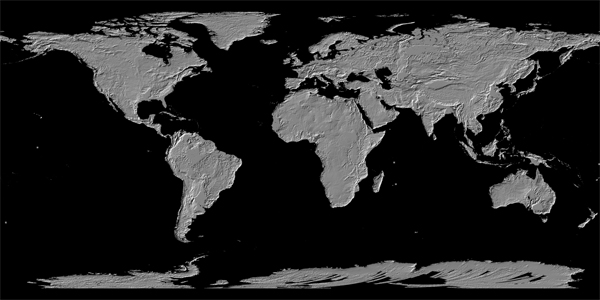
\includegraphics[width=\textwidth]{./charpter2/terrian/world_dem_2d.jpg}
        \caption{平面经纬度地形}
        \label{fig:world_dem_2d}
    \end{subfigure}
    \begin{subfigure}[b]{0.3\textwidth}
		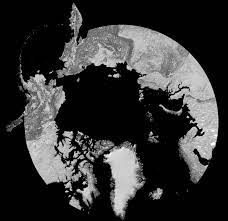
\includegraphics[width=\textwidth]{./charpter2/terrian/world_dem_3d.jpg}	
        \caption{球面经纬度地形}
        \label{fig:world_dem_3d}
    \end{subfigure}
\end{figure}

\begin{introduction}
	\item 那如何将平面的地形贴合到球面呢?
	\item 直接使用极坐标?
	\item 间接使用笛卡尔积坐标?
\end{introduction}

\subsection{椭球基本知识}
\begin{enumerate}
	\item 基本方程 
	\begin{equation}
		\frac{x^2}{a^2} + \frac{y^2}{b^2} + \frac{z^2}{c^2} = 1
	\end{equation}
	\item 扁率\footnote{扁率e = (a – c) / a = 1 / 298.257223563, 很多时候喜欢使用分母298来表示扁率}
	\begin{equation}
		e = \frac{a - c}{a} 
	\end{equation}
	\item 扁率以及长短轴的互相计算
	\begin{equation}
		c = a * (1 - e)
	\end{equation}
\end{enumerate}	


\begin{figure}[!htb]
	\centering
	\begin{subfigure}[b]{0.4\textwidth}
        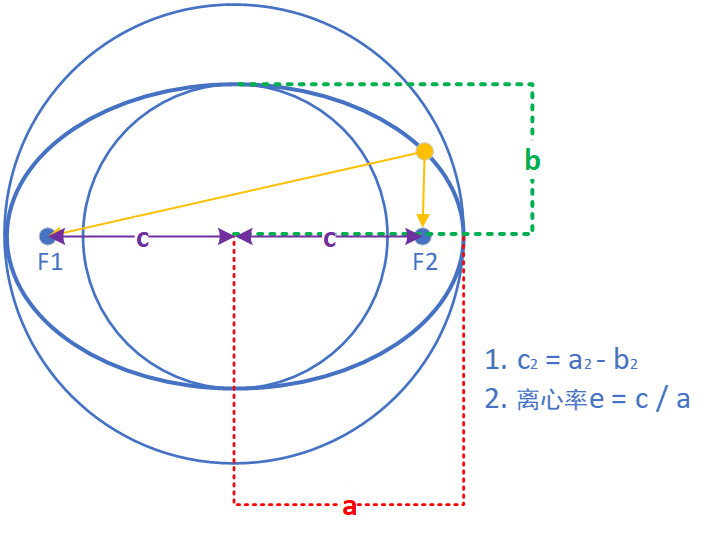
\includegraphics[width=\textwidth]{./charpter2/terrian/ellipsoid.png}
        \caption{椭圆基本理论知识}
    \end{subfigure}
    \begin{subfigure}[b]{0.5\textwidth}
		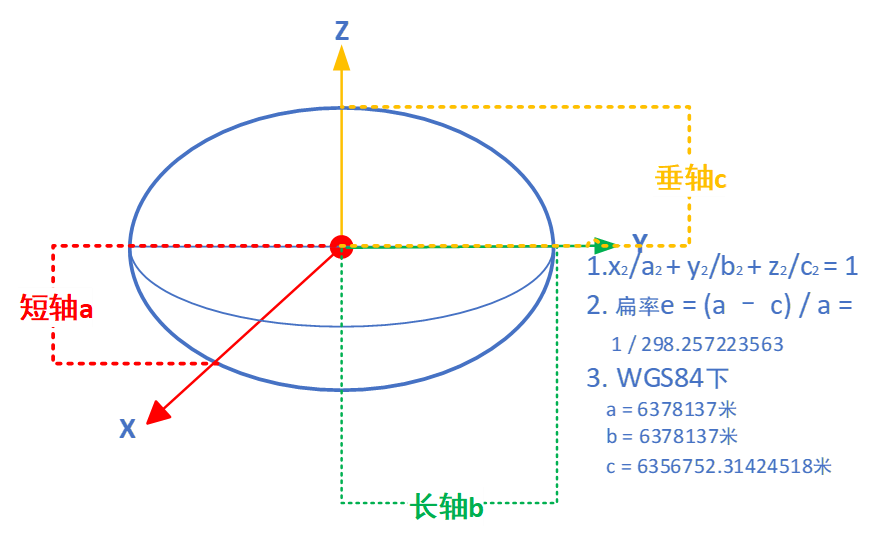
\includegraphics[width=\textwidth]{./charpter2/terrian/ellipsoid_wgs84.png}	
        \caption{椭球基本理论知识}
    \end{subfigure}
\end{figure}

\subsection{地形核心原理}
核心原理是先根据经纬度计算出\hyperref[sec:ellipsoid-surface]{\textbf{椭球表面}}上一个点对应的笛卡尔积,然后再追加加该点对应的高度h的向量,就可以得到椭球坐标系下\hyperref[sec:ellipsoid-dem-height]{\textbf{地形高程}}的真实迪卡坐标值。
\begin{note}
	这段话开始不理解没关系,后面会极为详细的解析对应的空间原理
\end{note}
\begin{figure}[!htb]
	\centering
	\begin{subfigure}[b]{0.4\textwidth}
        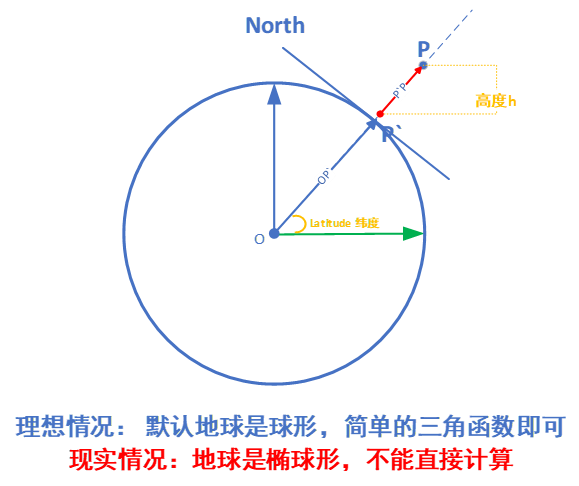
\includegraphics[width=\textwidth]{./charpter2/terrian/idea_state.png}
        \caption{理想情况}
        \label{fig:idea_state}
    \end{subfigure}
    \begin{subfigure}[b]{0.5\textwidth}
		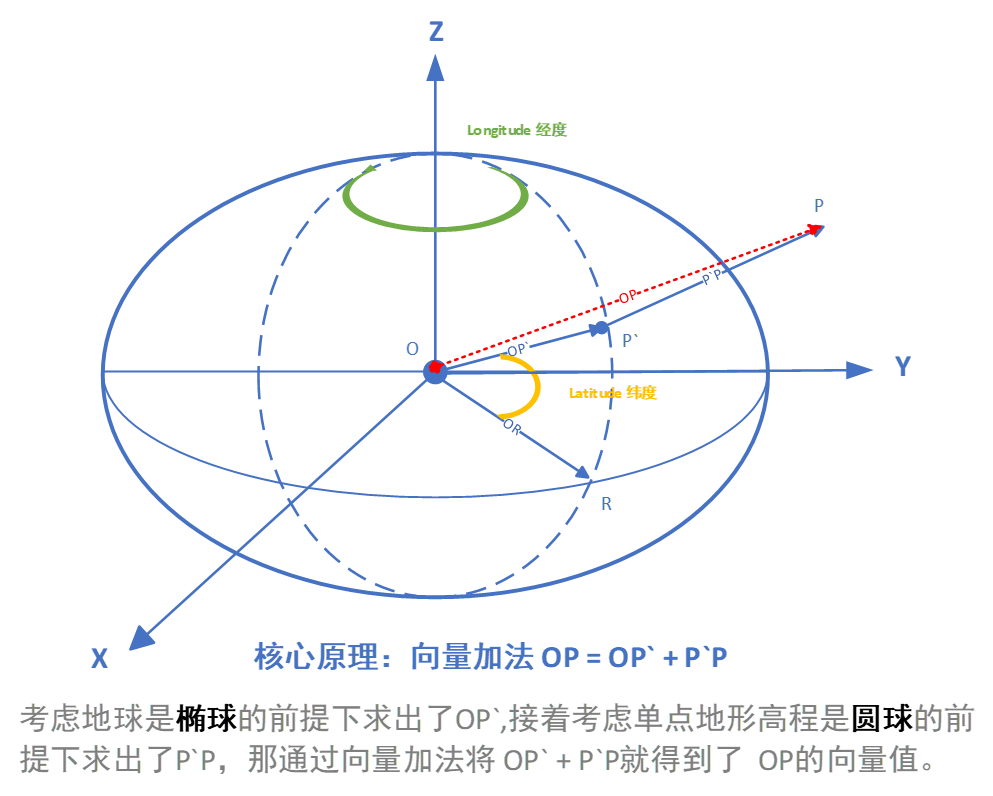
\includegraphics[width=\textwidth]{./charpter2/terrian/actual_state.png}	
        \caption{现实情况}
        \label{fig:actual_state}
    \end{subfigure}
\end{figure}

\subsection{椭球表面原理}
\label{sec:ellipsoid-surface}

\begin{figure}[!htb]
	\centering
	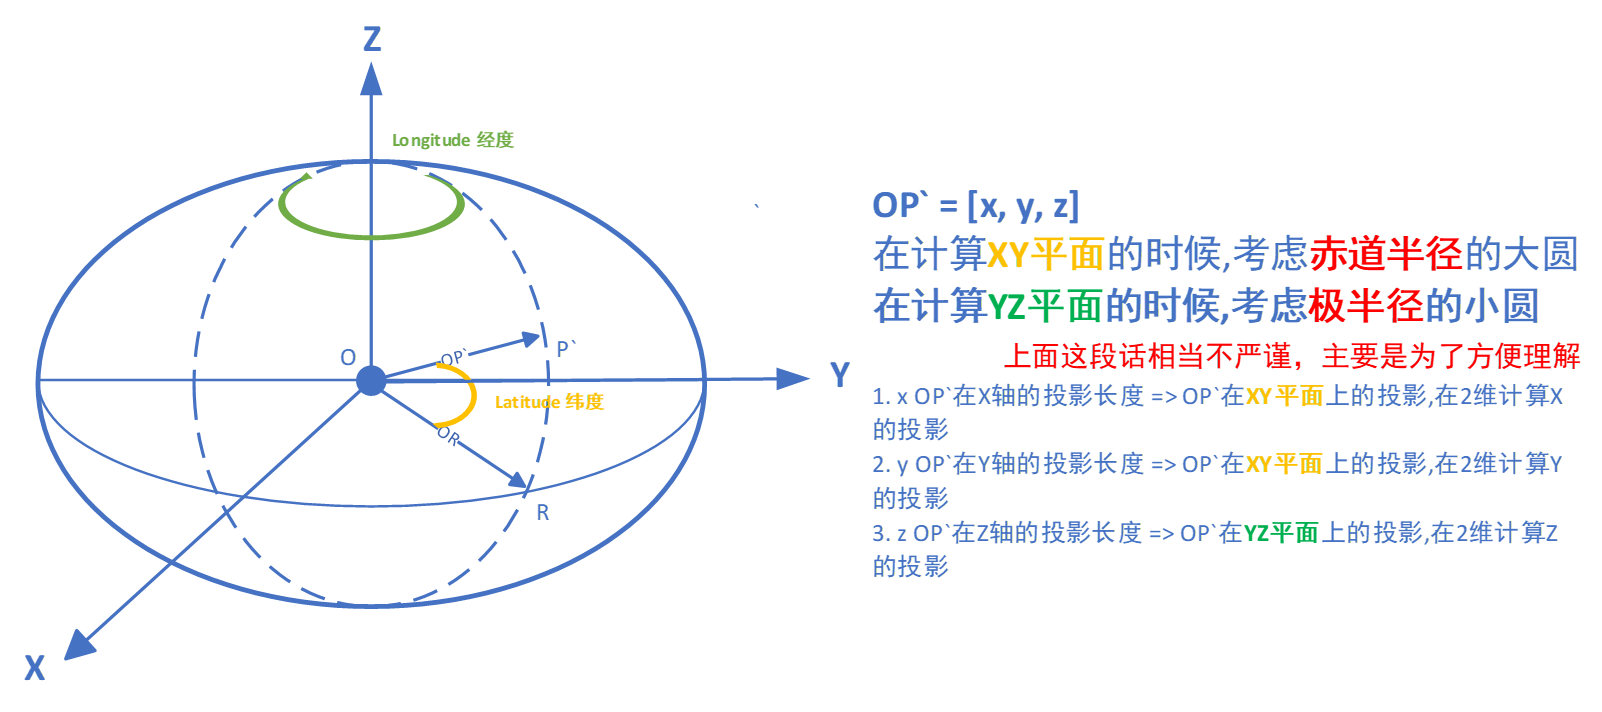
\includegraphics[width=1.0\textwidth]{./charpter2/terrian/ellipsoid_surface_xyz.png}
\end{figure}

\subsubsection{赤道半径平面计算}
\begin{figure}[!htb]
	\centering
	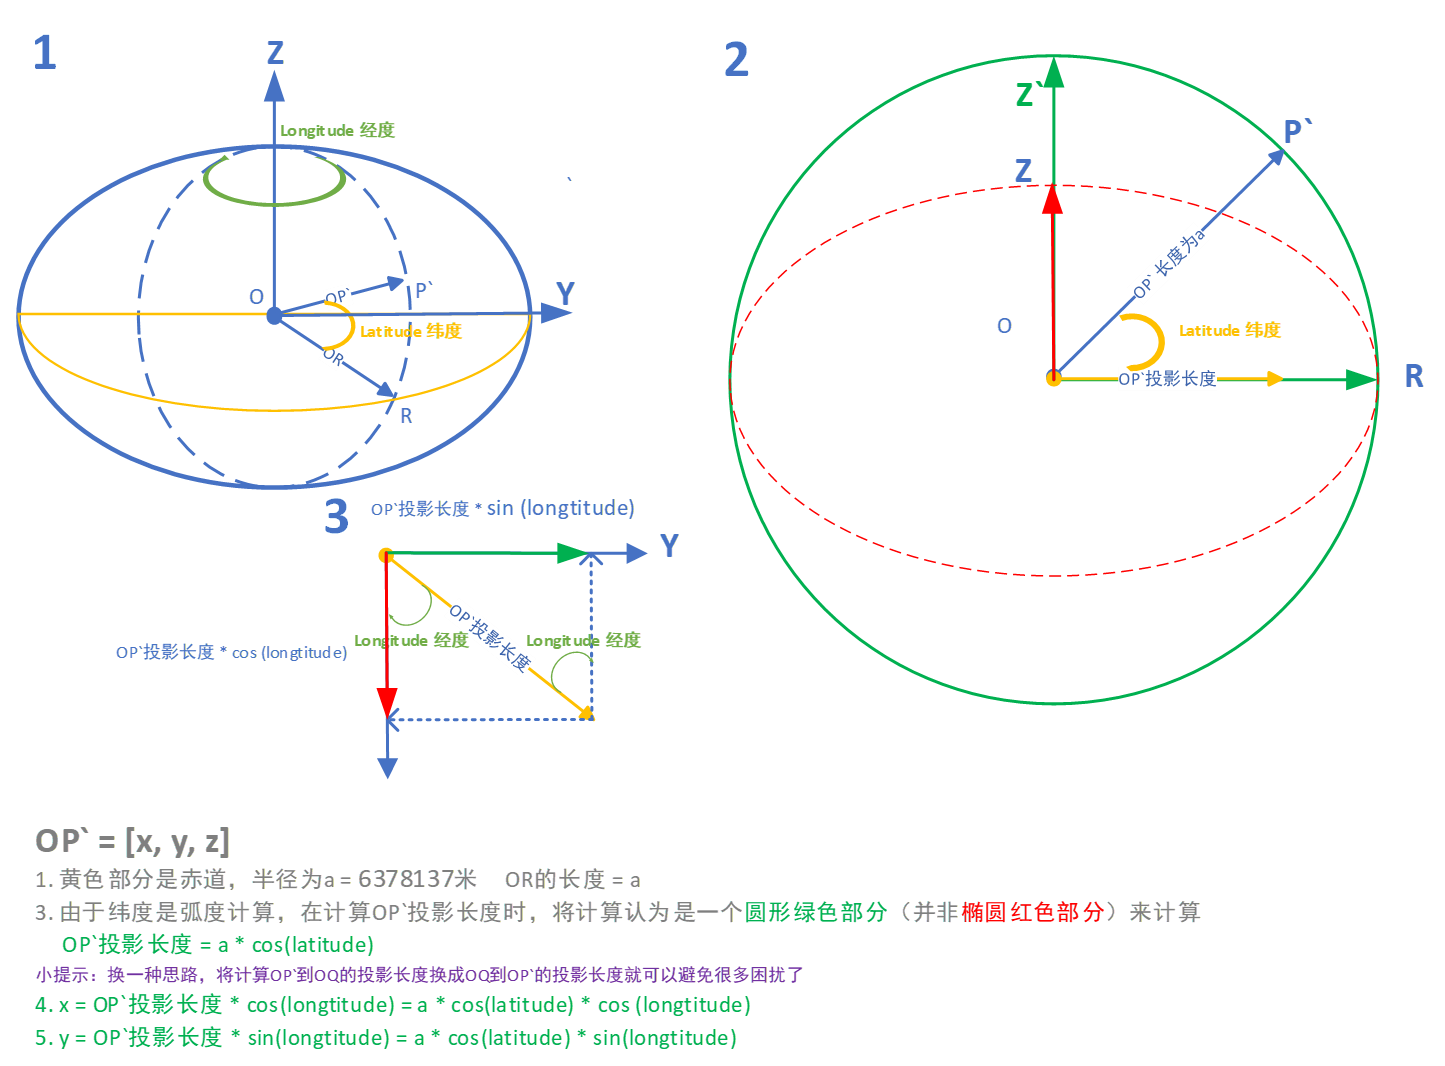
\includegraphics[width=1.0\textwidth]{./charpter2/terrian/ellipsoid_surface_equator.png}
\end{figure}
\subsubsection{极半径平面计算}
\begin{figure}[!htb]
	\centering
	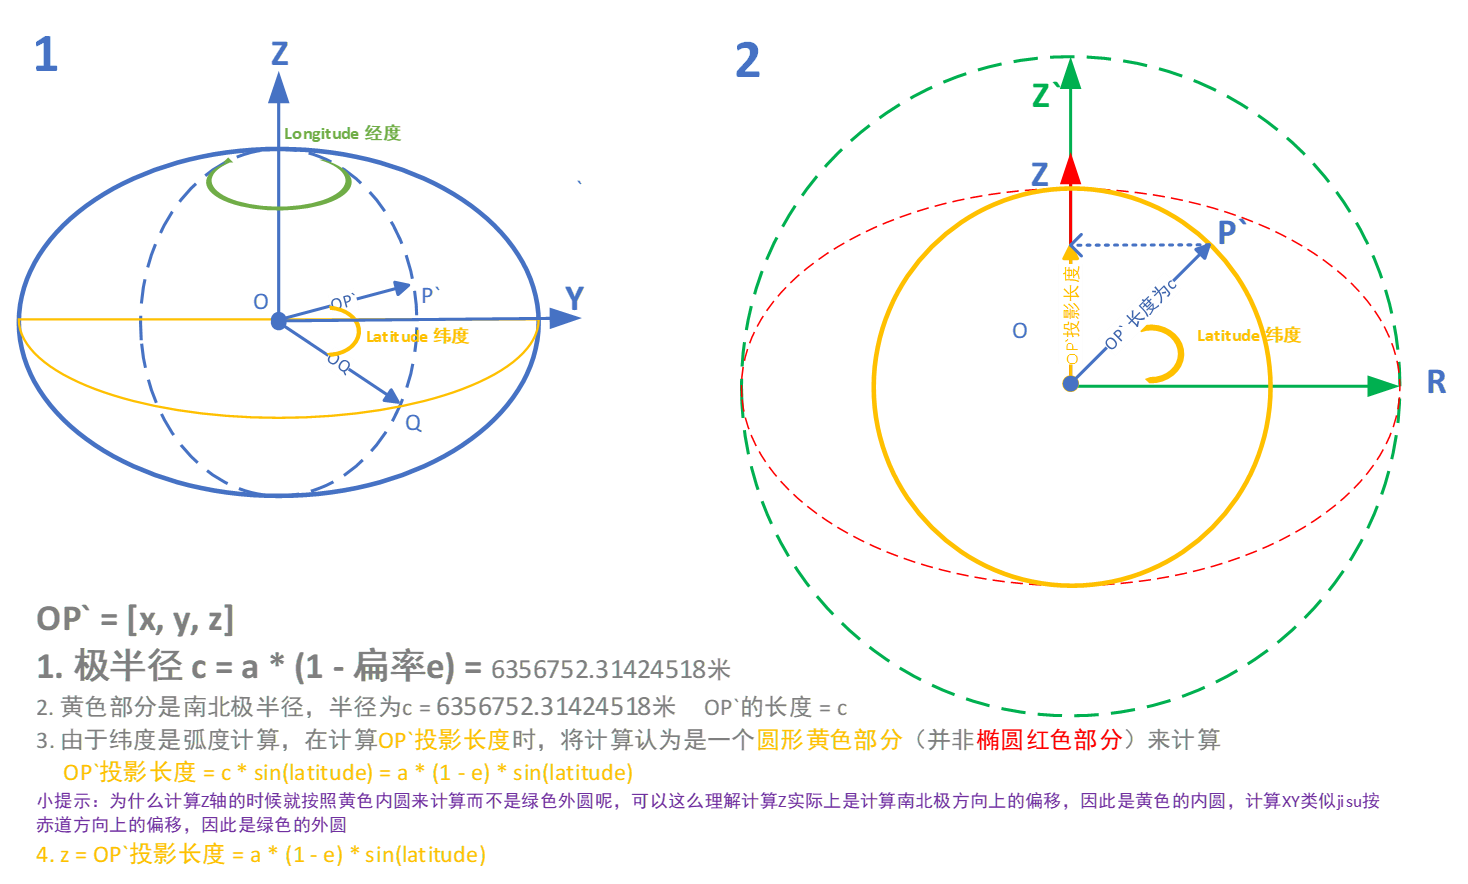
\includegraphics[width=1.0\textwidth]{./charpter2/terrian/ellipsoid_surface_pole.png}
\end{figure}

\subsection{地形高程原理}
\label{sec:ellipsoid-dem-height}
\begin{figure}[!htb]
	\centering
	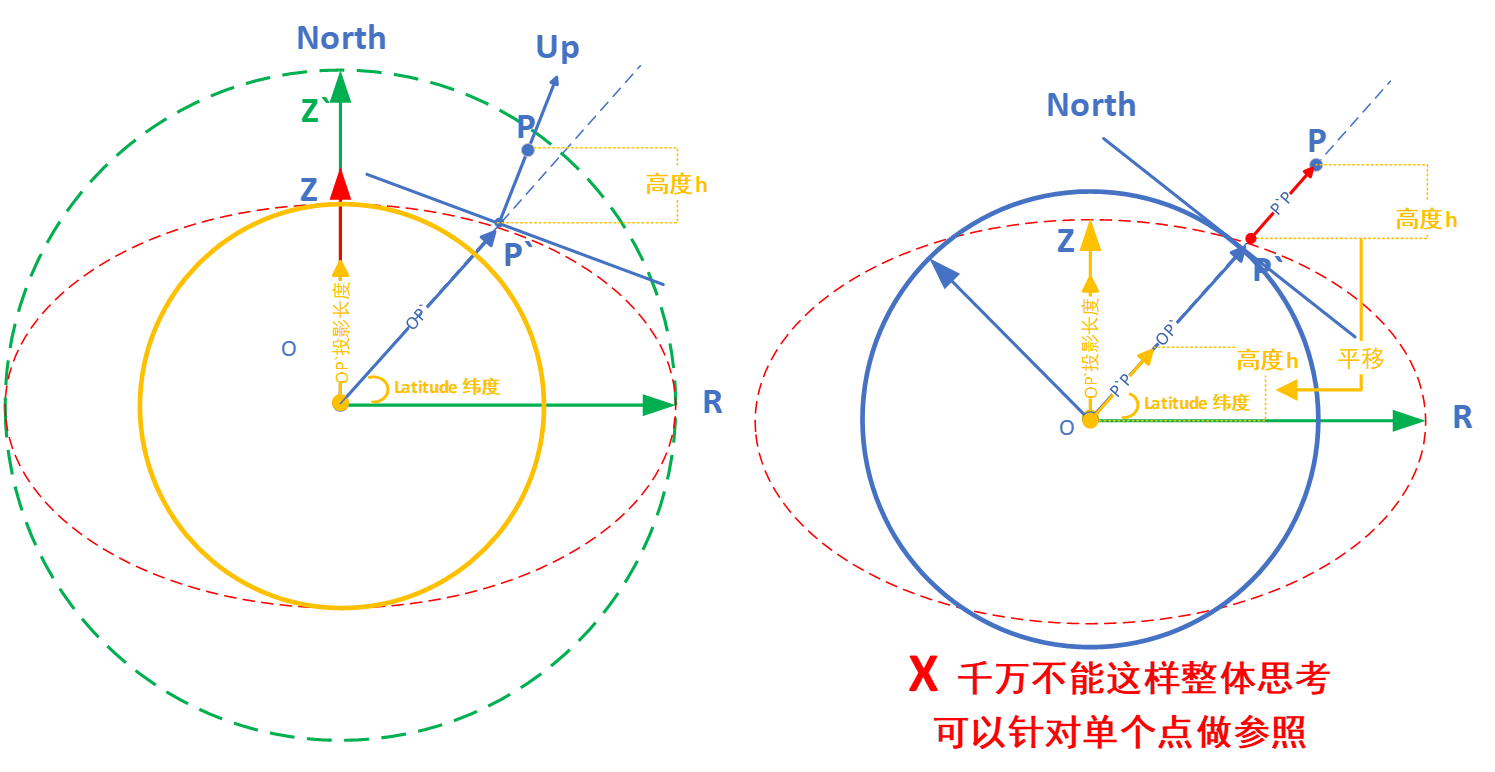
\includegraphics[width=1.0\textwidth]{./charpter2/terrian/ellipsoid_dem_height_1.png}
\end{figure}

\begin{equation}
	\overrightarrow{P'P} = \begin{bmatrix} x \\[0.3em] y \\[0.3em] z  \end{bmatrix} 
\end{equation}
\begin{enumerate}
	\item 之前计算OP'是把地球当作一个椭球来计算的得到的公式如下:
	\begin{enumerate}
		\item x = 赤道半径 * cos(longtitude) = a * cos(latitude) * cos (longtitude)
		\item y = 赤道半径 * sin(longtitude) = a * cos(latitude) * sin(longtitude)
		\item z = 极半径 * sin(latitude) = a * (1 - e) * sin(latitude)
	\end{enumerate}
	\item 现在我们思考一下,地球是一个椭球,某个点对应地形的高度在采集时候实际上是认为该点对应地表向下延申直至地心,其经纬度都和改地表点保持一致。在只考虑单点以及对应的参心圆球前提下,将红色P'P平移到黄色P'P上,就可以直接套用上面的公式
	\begin{enumerate}
		\item x = 地形高度 * cos(longtitude)  = h * cos(latitude) * cos (longtitude)
		\item y = 地形高度 * sin (longtitude)  = h * cos(latitude) * sin (longtitude)
		\item z = 地形高度 * sin (latitude)       = h * sin(latitude)
	\end{enumerate}
	\item 之前通过考虑地球是椭球的前提下求出了OP',接着考虑单点地形高程是圆球的前提下求出了P'P,那通过向量加法将 OP' + P'P就得到了  OP的向量值。
	\item 此时OP的物理意义是考虑地球是椭球的客观前提下,计算出来的地形对应的其在椭球坐标系下的笛卡尔坐标值。
\end{enumerate}

\subsection{公式汇总}
\begin{enumerate}
	\item lat = latitude = 纬度
	\item lng = longtiude = 经度
	\item e = 扁率
	\item a = 长轴(赤道半径) = 6378137米
	\item c = 短轴(极半径) = 6356752.31424518米
	\item h = height = 地形高度(每个点对应的地形灰度值都各不相同)
\end{enumerate}

\begin{equation}
	\overrightarrow{OP'} = \begin{bmatrix} x \\[0.3em] y \\[0.3em] z  \end{bmatrix} = 
	\begin{bmatrix} a \times{} \cos{lat} \times{} \cos{lng}  \\[0.3em]
	a \times{} \cos{lat} \times{} \sin{lng} \\[0.3em]
	a \times{} ( 1 - e) \times{} \sin{lat} \end{bmatrix}	
\end{equation}
\begin{equation}
	\overrightarrow{P'P} = \begin{bmatrix} x \\[0.3em] y \\[0.3em] z  \end{bmatrix} = 
	\begin{bmatrix} h \times{} \cos{lat} \times{} \cos{lng}  \\[0.3em]
	h \times{} \cos{lat} \times{} \sin{lng} \\[0.3em]
	h \times{} \sin{lat} \end{bmatrix}	
\end{equation}	
\begin{equation}
	\overrightarrow{OP} = \overrightarrow{OP'} + \overrightarrow{P'P} = 
	\begin{bmatrix} (a + h) \times{} \cos{lat} \times{} \cos{lng}  \\[0.3em]
		(a + h) \times{} \cos{lat} \times{} \sin{lng} \\[0.3em]
		(a \times{} ( 1 - e) + h) \times{} \sin{lat} \end{bmatrix}	
\end{equation}	

\subsection{生命周期}
\begin{introduction}
	\item 基础框架生命周期
	\item MapGIS地形如何在基础生命周期中工作?
	\item STK地形如何在基础生命周期中工作?
\end{introduction}

\textbf{基础框架生命周期}

\begin{enumerate}
	\item QuadtreePrimitive.processSinglePriorityLoadQueue();
	\item GlobeSurfaceTileProvider.loadTile();
	\item GlobeSurfaceTile.processStateMachine()->requestTileGeometry()->doRequest()
	\item requestPromise = terrainProvider.requestTileGeometry(x, y, level, request); 这一步的terrainProvider使用初始化的地形,如果是IGS就是MapGISTerrainProvider。
\end{enumerate}

\begin{tikzpicture}
	\begin{umlseqdiag}
		\umlobject[class=QuadtreePrimitive]{QT}
		\umlobject[class=GlobeSurfaceTileProvider]{GSTP}
		\umlobject[class=GlobeSurfaceTile]{GST}
		\umlobject[class=TerrainProvider]{TP}
		\begin{umlcall}[op=processSinglePriorityLoadQueue]{QT}{GSTP}
			\begin{umlcall}[op=loadTile]{GSTP}{GST}
				\begin{umlcallself}[op=processStateMachine]{GST}
				\end{umlcallself}
				\begin{umlcallself}[op=requestTileGeometry]{GST}
				\end{umlcallself}
				\begin{umlcall}[op=doRequest]{GST}{TP}
					\begin{umlcallself}[op=requestTileGeometry,fill=green]{TP}
					\end{umlcallself}
				\end{umlcall}	
			\end{umlcall}
		\end{umlcall}
	\end{umlseqdiag}
\end{tikzpicture}

\subsubsection{MapGIS地形-MTP}
上一章节中提到的terrainProvider.requestTileGeometry,如果采取MapGIS的地形,则进入MapGISTerrainProvider的工作逻辑,如果是STK地形则进入CesiumTerrainProvider的逻辑。

\begin{tikzpicture}
	\begin{umlseqdiag}
		\umlobject[class=MapGISTerrainProvider]{MTP}
		\umlobject[class=全局函数]{G}
		\begin{umlcallself}[op=requestTileGeometry]{MTP}
		\end{umlcallself}
		\begin{umlcallself}[type=asynchron,op=requestTileGeometryForMapgis,fill=green,return=promise]{MTP}
			\begin{umlcall}[op=createHeightmapTerrainData]{MTP}{G}
				\begin{umlcallself}[op=判断是否是整形/浮点型数据]{G}
				\end{umlcallself}		
				\begin{umlcallself}[op=判断是否开启法线功能]{G}
				\end{umlcallself}		
				\begin{umlcallself}[op=判断是否激活水面]{G}
				\end{umlcallself}		
			\end{umlcall}	
		\end{umlcallself}
	\end{umlseqdiag}
\end{tikzpicture}

\subsubsection{MapGIS地形-法线}
|----4226 * 4 = 16904 ----|
\begin{enumerate}
	\item MTP法向地形头文件结构,偏移值\textbf{offset}为\begin{equation} offset = (height \times width + 1) \times float32 = (65 \times 65 + 1) \times 4 = 16904 (bytes) \end{equation}
	\item MTP法向地形头文件结构,存储区域为\textbf{content}为\begin{equation} content = (height \times width ) \times 2 \times unit8 = (65 \times 65 ) \times 2 \times 1 = 8450 (bytes) \end{equation}
\end{enumerate}

\begin{tikzpicture}[scale=.9,every node/.style={minimum size=1cm},on grid]
		
	\begin{scope}[
    	yshift=-25,every node/.append style={
    	yslant=0.5,xslant=-1},yslant=0.5,xslant=-1
    	             ]
    	\fill[white,fill opacity=.9] (0,0) rectangle (6,6);
    	\draw[step=2mm, black] (0.25,0.25) grid (5.75,5.75);
		\draw[black,very thick] (0.25,0.25) rectangle (5.75,5.75);
    	\draw[blue,dashed] (0,0) rectangle (6,6);
		\fill[blue] (0.25,0.25) rectangle (0.4,0.4);
		\draw [fill=lime](6,0) circle (.1);
		\draw [fill=lime](0,6) circle (.1);
		\draw [fill=lime](6,6) circle (.1);
		\draw [fill=lime](0,0) circle (.1);
    \end{scope}

	\begin{scope}[
    	yshift=60,every node/.append style={
    	yslant=0.5,xslant=-1},yslant=0.5,xslant=-1
    	             ]
    	\fill[white,fill opacity=.9] (0,0) rectangle (6,6);
    	\draw[step=2mm, black] (0.25,0.25) grid (5.75,5.75);
		\draw[black,very thick] (0.25,0.25) rectangle (5.75,5.75);
		\fill[red] (0.25,0.25) rectangle (0.4,0.4);
		\draw [fill=lime](5.75,0.25) circle (.05);
		\draw [fill=lime](0.25,0.25) circle (.05);
		\draw [fill=lime](0.25,5.75) circle (.05);
		\draw [fill=lime](5.75,5.75) circle (.05);
    \end{scope}	

	\draw[-latex,thick] (6,4) node[right]{$\mathsf{skirt:1px}$} to[out=180,in=90] (4,3);
	\draw[-latex,thick] (6,2) node[right]{$\mathsf{center:65px}$} to[out=180,in=90] (4,2);
	\draw[-latex,thick,red] (6,5) node[right]{$\mathsf{ i * 65 + j}$} to[out=180,in=90] (0,2.5);
	\draw[-latex,thick,blue] (6,-0.5) node[right]{$\mathsf{  (i + skirt) * (2 * skirt + center ) + j + skirt;}$} to[out=180,in=90] (0,-0.5);
	\fill[black,font=\footnotesize]
        (-5,0) node {MapGIS-IGServer-Normal}
        (-5,7) node {Cesium-Encode-Normal};
\end{tikzpicture}

\subsubsection{MapGIS地形-水面}
\begin{enumerate}
	\item MTP水面地形实际上是通过高程来计算出水面,因此数据区使用的就是地形的数据区
	\item MTP水面地形头文件结构,偏移值\textbf{offset}为\begin{equation} offset = height_{offset} = 0 (bytes)\end{equation}
	\item MTP水面地形头文件结构,存储区域为\textbf{content}为\begin{equation} content = (height \times width ) \times unit8 = (65 \times 65 ) \times 1 = 4225 (bytes) \end{equation}
\end{enumerate}

\begin{tikzpicture}[scale=.9,every node/.style={minimum size=1cm},on grid]
	\begin{scope}[
    	yshift=60,every node/.append style={
    	yslant=0.5,xslant=-1},yslant=0.5,xslant=-1
    ]
    	\fill[white,fill opacity=.9] (0,0) rectangle (6,6);
    	\draw[step=2mm, black] (0,0) grid (6,6);
		\draw[black,very thick] (0,0) rectangle (6,6);
		\draw[step=2mm, red] (2,2) grid (3,0);
		\draw[step=2mm, green] (2,2) grid (3,3);
		\draw [fill=lime](6,0) circle (.05);
		\draw [fill=lime](0,6) circle (.05);
		\draw [fill=lime](0,0) circle (.05);
		\draw [fill=lime](6,6) circle (.05);
    \end{scope}

	\draw[-latex,thick,red] (4,3) node[right]{$\mathsf{ zMin > height | height > zMin + waterHeight }$} to[out=180,in=90] (2,4);
	\draw[-latex,thick,green] (5,7) node[right]{$\mathsf{ zMin < height < zMin + waterHeight}$} to[out=180,in=90] (0,5);
\end{tikzpicture}

\begin{equation}
	f(height, zmin, waterheight) =
		\begin{cases}
			255       & \quad \text{if } zmin < height < zmin + waterheight\\
			0         & \quad \text{else } \text{其他情况}
		\end{cases}
\end{equation}

\subsubsection{Cesium地形-CTP}

\subsubsection{地形分析}
\begin{enumerate}
	\item 地形等值面(等值线)
	\item 坡度坡向分析
\end{enumerate}


\section{栅格瓦片}
\label{sec:cesium-raster}
栅格瓦片是依托于地形服务之上的一层覆盖物,如果把地形比作看不见的或者灰度高度。那么栅格就是贴合在地形上的一层覆盖物。

\begin{introduction}
	\item 等分弧秒投影瓦片
	\item Web墨卡托投影瓦片
	\item 自定义投影+自定义裁图瓦片
\end{introduction}

\subsection{核心原理}
%后面有空还是看看GlobeSurfaceTileProvider这一块的原理把%
\begin{enumerate}
	\item 首先整个地球(GlobeSurfaceTile)在初始化(initialize)的时候,会默认设置一个地形(terrainProvider)和一组栅格瓦片(imageryLayerCollection,默认至少包含一个基础的栅格瓦片底图)。
	\item 当整个环境准备好了以后,四叉树开始请求数据以后,开始准备瓦片的工作\begin{lstlisting}
		GlobeSurfaceTile.initialize = function (tile, terrainProvider, imageryLayerCollection) {
			var surfaceTile = tile.data;
			if (tile.state === QuadtreeTileLoadState.START) {
				prepareNewTile(tile, terrainProvider, imageryLayerCollection);
				tile.state = QuadtreeTileLoadState.LOADING;
			}
		};\end{lstlisting}
	\item 瓦片准备工作的步骤是先保证地形瓦片的存在,如果当前地形瓦片不存在,则向上其父级获取存在的瓦片临时作为当前地形瓦片来使用。然后遍历所有的栅格瓦片图层,每层各自请求对应的瓦片。
		\begin{lstlisting}
		function prepareNewTile(tile, terrainProvider, imageryLayerCollection) {
			var available = terrainProvider.getTileDataAvailable(tile.x, tile.y, tile.level);
		
			if (!defined(available) && defined(tile.parent)) {
				var parent = tile.parent;
				var parentSurfaceTile = parent.data;
				if (defined(parentSurfaceTile) && defined(parentSurfaceTile.terrainData)) {
					available = parentSurfaceTile.terrainData.isChildAvailable(parent.x, parent.y, tile.x, tile.y);
				}
			}
		
			if (available === false) {
				// 如果该地形瓦片是无效,立刻标记为FAILED并向上采样
				tile.data.terrainState = TerrainState.FAILED;
			}
		
			// 将栅格瓦片贴合到地形瓦片上
			for (var i = 0, len = imageryLayerCollection.length; i < len; ++i) {
				var layer = imageryLayerCollection.get(i);
				if (layer.show) {
					layer._createTileImagerySkeletons(tile, terrainProvider);
				}
			}
		}	
		\end{lstlisting}
		\item 由于地形一般都是经纬度坐标和切分方式,而栅格瓦片主流的有Web墨卡托投影(航海-电子底图)、等分弧秒投影(天地图-自然椭球)、高斯投影(自然资源-局部范围保证形变较小)甚至是自定义投影。因此不能保证每个经纬度的地形瓦片的行列号和栅格都是一一对应,因此需要有一个换算公式来进行对应的根据地形的范围来请求对应的栅格瓦片的行列号的公式。该公式就记录在createTileImagerySkeletons函数中。
		\item 上面换算公式的核心部分 一言以蔽之就是: 
		\begin{enumerate}
			\item 先通过当前栅格瓦片图层的范围和当前栅格瓦片数据源的范围进行求交分析,将空间范围缩小到有效范围内部。然后把得到的范围再和该地形瓦片的空间范围进一步求交可以得出本张瓦片(地形和栅格共同作用下)真正有效的瓦片范围。
			\item 
		\end{enumerate}
\end{enumerate}

\begin{tikzpicture}
	\begin{umlseqdiag}
		\umlobject[class=GlobeSurfaceTile]{GST}
		\umlobject[class=ImageryLayer]{IL}
		\umlobject[class=TilingScheme]{TS}
		\umlobject[class=CustomTilingScheme]{CTS}
		\begin{umlcallself}[op=initialize]{GST}
			\begin{umlcall}[op=prepareNewTile]{GST}{IL}
				\begin{umlcall}[op=createTileImagerySkeletons]{IL}{TS}	
				\end{umlcall}
			\end{umlcall}
		\end{umlcallself}
	\end{umlseqdiag}
\end{tikzpicture}


\section{M3D}
\subsection{核心入口}
	单体建筑生长.mcj
\begin{enumerate}
	\item 文件格式 \textbf{json}
	\item 文件编码 \textbf{GB2312}
\end{enumerate} 

\textbf{服务示例}
http://192.168.199.71:8089/igs/rest/services/CIMyanshi/BIM单体建筑生长V13/M3dServer

\subsubsection{索引文件MCJ}
\begin{lstlisting}
{
	"asset": "Zondy Inc.",
	"version": "2.0",
	"dataName": "高级住所模型",
	"guid": "2B444694130E4FD699A4791023735A76",
	"compressType": "0",
	"spatialReference": "WGS84",
	"treeType": "AttTree",
	"lodType": "ADD",
	"boundingVolume": {
		"boundingBox": {
			"left": 2.114275787341435,
			"top": 0.5036272461576443,
			"right": 2.1142832158691697,
			"bottom": 0.5036250037611653,
			"minHeight": -0.3499998794868589,
			"maxHeight": 13.259142253547909
		}
	},
	"position": {
		"x": 121.1392921528815,
		"y": 28.85565141287461,
		"z": 6.454571067811866
	},
	"rootNode": {
		"uri": "rootNode.json"
	},
	"fieldInfo": [ // 后期针对number型,完全可以学习cesiumlab增加一个最大最小的范围值
		{
			"alias": "alias",
			"name": "mpLayer",
			"type": "uint64",
			"size": 4
		}
	]
}
\end{lstlisting}

\subsubsection{根节点rootNode}
\begin{lstlisting}
{
    "name": "rootNode",
    "lodLevel": 0,
    "boundingVolume": { https://github.com/CesiumGS/3d-tiles/tree/main/specification#tileboundingvolume-white_check_mark
        "boundingBox": { // 既不是 Region 也不是 Box 也不是 Box 对应的转换规则可能需要说明一下,感觉像是弧度坐标
            "left": 2.114275787341435,
            "top": 0.5036272461576443,
            "right": 2.1142832158691697,
            "bottom": 0.5036250037611653,
            "minHeight": -0.3499998794868589,
            "maxHeight": 13.259142253547909
        }
    },
    "lodMode": "pixel", // 找不到3dtiles的描述,对应的枚举可能需要说明一下
    "lodType": "ADD",  // https://github.com/CesiumGS/3d-tiles/tree/main/specification#tilerefine
    "lodError": 10000.0, // https://github.com/CesiumGS/3d-tiles/tree/main/specification#tilesetgeometricerror-white_check_mark
    "childrenNode": [ // https://github.com/CesiumGS/3d-tiles/tree/main/specification#tilechildren
        {
            "boundingVolume": {
                "boundingBox": {
                    "left": 2.114275787341435,
                    "top": 0.5036272461576443,
                    "right": 2.1142832158691697,
                    "bottom": 0.5036250037611653,
                    "minHeight": -0.34999987948685887,
                    "maxHeight": 13.259142253547907
                }
            },
            "lodError": 10000.0,
            "uri": "./node/0/0.json"
        }
    ]
}
\end{lstlisting}

\subsubsection{内容节点contentNode}
\begin{figure}[!htb]
    \centering
    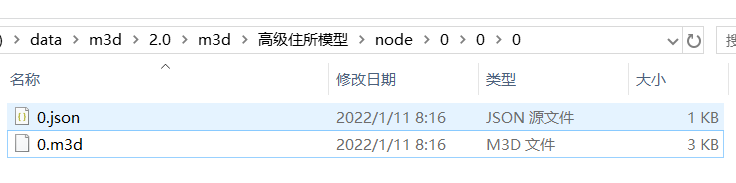
\includegraphics[width=0.9\textwidth]{./charpter2/m3d/m3d_content_json.png}
  \end{figure}
\begin{lstlisting}
	{
		"name": "2021-1-1",
		"lodLevel": 3,
		"boundingVolume": {
			"boundingBox": {
				"left": 2.114277136002482,
				"top": 0.5036251993010383,
				"right": 2.114277566540517,
				"bottom": 0.5036250263785022,
				"minHeight": 1.0846084877848626,
				"maxHeight": 4.6010056445375089
			}
		},
		"lodMode": "pixel",
		"lodType": "ADD",
		"lodError": 10000.0,
		"parentNode": {
			"uri": "../0.json"
		},
		"tileDataInfoIndex": 0,  // 这个值大部分情况是0,具体的意思是什么??
		"tileDataInfoList": [
			{
				"tileData": { // https://github.com/CesiumGS/3d-tiles/tree/main/specification#transforms
					"uri": "0.m3d"
				},
				"geometry": {
					"blobType": "glbx", // 感觉是用来做子分类的
					"uri": "./geometry/0.glbx",
					"geometryType": "Surface" // 这个的枚举可能也得说明一下了
				},
				"dataType": "Model" 
			}
		]
	}
\end{lstlisting}

\subsection{目录代码}
Source/MapGIS/M3dLayer/\textbf{MapGISM3DSet.js}
\begin{enumerate}
	\item 关键构造函数 
	\begin{lstlisting}
		// 用于访问 igs
		this._isIGServer = defaultValue(options.igserver, false);
		this._layerRenderIndex = defaultValue(options.layerRenderIndex, 0); // 渲染图层索引,这个可以具体一点不,有点抽象
		this._layerIndex = defaultValue(options.layerIndex, 0); // 图层索引(用来标识组图层的概念)
		this._gdbpUrl = defaultValue(options.gdbpUrl, ''); // 原始数据在gdb中的数据
		this._name = undefined; // 图层名
		this._guid = undefined; // 图层的guid
		this._extLayer = undefined; // 这里先为 挂接单体化预留 用来绑定单体化所用到的附加图层
		this._version = undefined;

		//fgy 20210917 update
		this._pickTextureCoordinate = defaultValue(options.pickTextureCoordinate, false);
		this._cacheState = CacheState.UNKNOW;
		this._useIDB = defaultValue(options.useIDB, false);
		this._key = '_' + this._layerRenderIndex + '_' + this.layerIndex;
		this._indexedRequest = defaultValue(options.indexedDBRequest, undefined);
		this._maxCacheLevel = defaultValue(options.maxCacheLevel, 3);
		this._pickedColor = Color.YELLOW.withAlpha(0.5);
		this._attributeNumber = 0.0;

		//ljy Pbr param
		this._pbrParam = defaultValue(options.pbrParam, undefined);

		//ljy Instances
		// 这个地方感觉是原来的文件服务 xxx.mcj做字符替换的,后面还需要吗? 这里需要一个实际数据才能明白这个逻辑
		var file_name = options.url.replace(/(.*\/)*([^.]+).*/gi, '$2');
		var FileExt = options.url.replace(/.+\./, '');
		this._sharedUrl = options.url.replace(file_name + '.' + FileExt, 'shared/');
	\end{lstlisting}
\end{enumerate}